\section{Background and Motivation}

In this section, we discuss the hardware and software stacks in ML training and serving platforms. We explore the possible failure handling solutions and examine why they can be ill-suited to address network failures.

\subsection{Hardware Stack and Common Failures }
\label{sec:bg-stack}

\noindent\textbf{Hardware stack in GPU Clusters.}
Modern GPU clusters employ a two-tier communication fabric that separates high-bandwidth intra-node communication from constrained inter-node links.\footnote{Examples include production LLM training clusters reported by Meta~\cite{gangidi2024rdma}, Alibaba~\cite{qian2024alibaba}, and others.}
Within a server node, GPUs are connected via NVLink or NVSwitch, providing hundreds of GB/s of bidirectional bandwidth and low latency between devices on the same node.
Between nodes, GPUs communicate through RDMA-capable NICs (e.g., InfiniBand or RoCE) attached to the host over PCIe.
Because a single NIC typically offers substantially less bandwidth than the intra-node fabric, production servers aggregate multiple NIC ``rails'' per node, and the effective inter-node connection between a pair of servers consists of several physical paths that may traverse different switch ports or even different ToR switches.
Recent designs, such as multi-plane fabrics~\cite{qian2024alibaba,oci-multiplanar,khashab2026high} and GPU servers with directly attached NICs, change how NICs connect to switches and GPUs; Appendix~\ref{app:discussion} discusses R2CC under these designs.
GPU buffers are exposed to these NICs via memory registration, allowing NICs to perform direct RDMA reads and writes on GPU memory without CPU-side copies, but only along links for which registration and queue pairs have been established.

\smallskip\noindent\textbf{Common hardware failures.}
Failures in this stack fall into three categories: GPU failures, intra-node link failures, and inter-node network failures. GPU failures include hardware, memory, or other errors that render a device unusable. Intra-node link failures are faults in the GPU fabric within a server. Inter-node network failures are faults that affect the available bandwidth or the set of network paths between two otherwise live GPU endpoints.

\smallskip\noindent\textbf{R2CC scope.}
As a CCL, R2CC targets \textbf{inter-node network failures} that change the available paths or bandwidth between live GPU endpoints, while at least one alternate path remains usable. This includes hard faults such as NIC, port, cable, or ToR-port failures, as well as gray failures, such as link flapping, that surface as transport errors. GPU failures that remove the compute endpoint, including rare cases where network faults co-occur with GPU failures~\cite{Revisiting_Reliability}, are out of scope; they are typically handled by training and inference frameworks. Intra-node link failures are also out of scope because proprietary protocols such as NVLink/NVSwitch lack a CPU/CCL-visible recoverable transport boundary, such as per-transfer completion/error reporting and replay state. Supporting such failures would require redesigning the intra-node transport protocol. Intra-node link failures are also not reported as frequent errors in the hardware stack. Additional discussion is provided in Appendix~\ref{app:failure-scope}.

\subsection{Software Stack}
\label{sec:bg-failures}
Figure~\ref{fig:layer} illustrates the software layering of distributed collective communication.

\smallskip\noindent\textbf{Framework layer.}
The ML framework layer owns the training or inference loop. Systems such as PyTorch~\cite{paszke2019pytorch}, DeepSpeed~\cite{rasley2020deepspeed}, and Megatron~\cite{shoeybi2019megatron} partition work across GPUs and maintain model or request state across iterations. They drive training steps such as forward, backward, and optimizer updates, or serving request steps such as prefilling and decoding~\cite{kwon2023efficient,agrawal2024taming,zhong2024distserve}. The framework delegates cross-GPU data movement to the CCL layer through collective or point-to-point operations.

\smallskip\noindent\textbf{CCL layer.}
The CCL layer implements the collective and point-to-point operations delegated from the framework. Libraries such as NCCL~\cite{NCCL}, RCCL~\cite{RCCL}, and UCCL~\cite{zhou2025extensible} organize the participating GPUs into channels and realize each collective as a ring or tree schedule. In a ring schedule, data is partitioned into chunks that circulate across GPUs, advancing one hop per step. For collectives such as Broadcast, ReduceScatter, or AllGather with input size $D$, each server sends and receives approximately $D$ bytes. AllReduce is commonly implemented as a ReduceScatter followed by an AllGather, resulting in 2D bytes of communication per server.

Each transfer step in CCL follows a specific performance-oriented protocol. In throughput-oriented protocols, bulk data transfer is decoupled from completion notification: the GPU processes data only after the receiver’s CPU observes a corresponding notification. In contrast, low-latency protocols embed both payload and progress metadata within the same transfer, allowing the GPU to consume data incrementally as it arrives. The CCL layer coordinates these transfers and drives communication progress.

\smallskip\noindent\textbf{RDMA verbs layer.}
The RDMA verbs layer provides the interface between the CCL and the network hardware. Inter-node communication is realized through queue pairs (QPs) established between endpoints. The CCL issues work requests (WRs) to initiate communication and polls completion queues (CQs) for work completions (WCs), which indicate progress or errors. Two operations are commonly used here: RDMA Write transfers data directly into a pre-registered remote GPU buffer without involving the receiver's CPU. RDMA Write with Immediate (WriteImm) additionally carries a small inline value, consumes a pre-posted receive request on the remote side, and generates a completion event to notify the receiver. These primitives enable high-throughput, low-overhead communication but provide only limited visibility into higher-level communication semantics.

\begin{figure}[t]
    \centering
    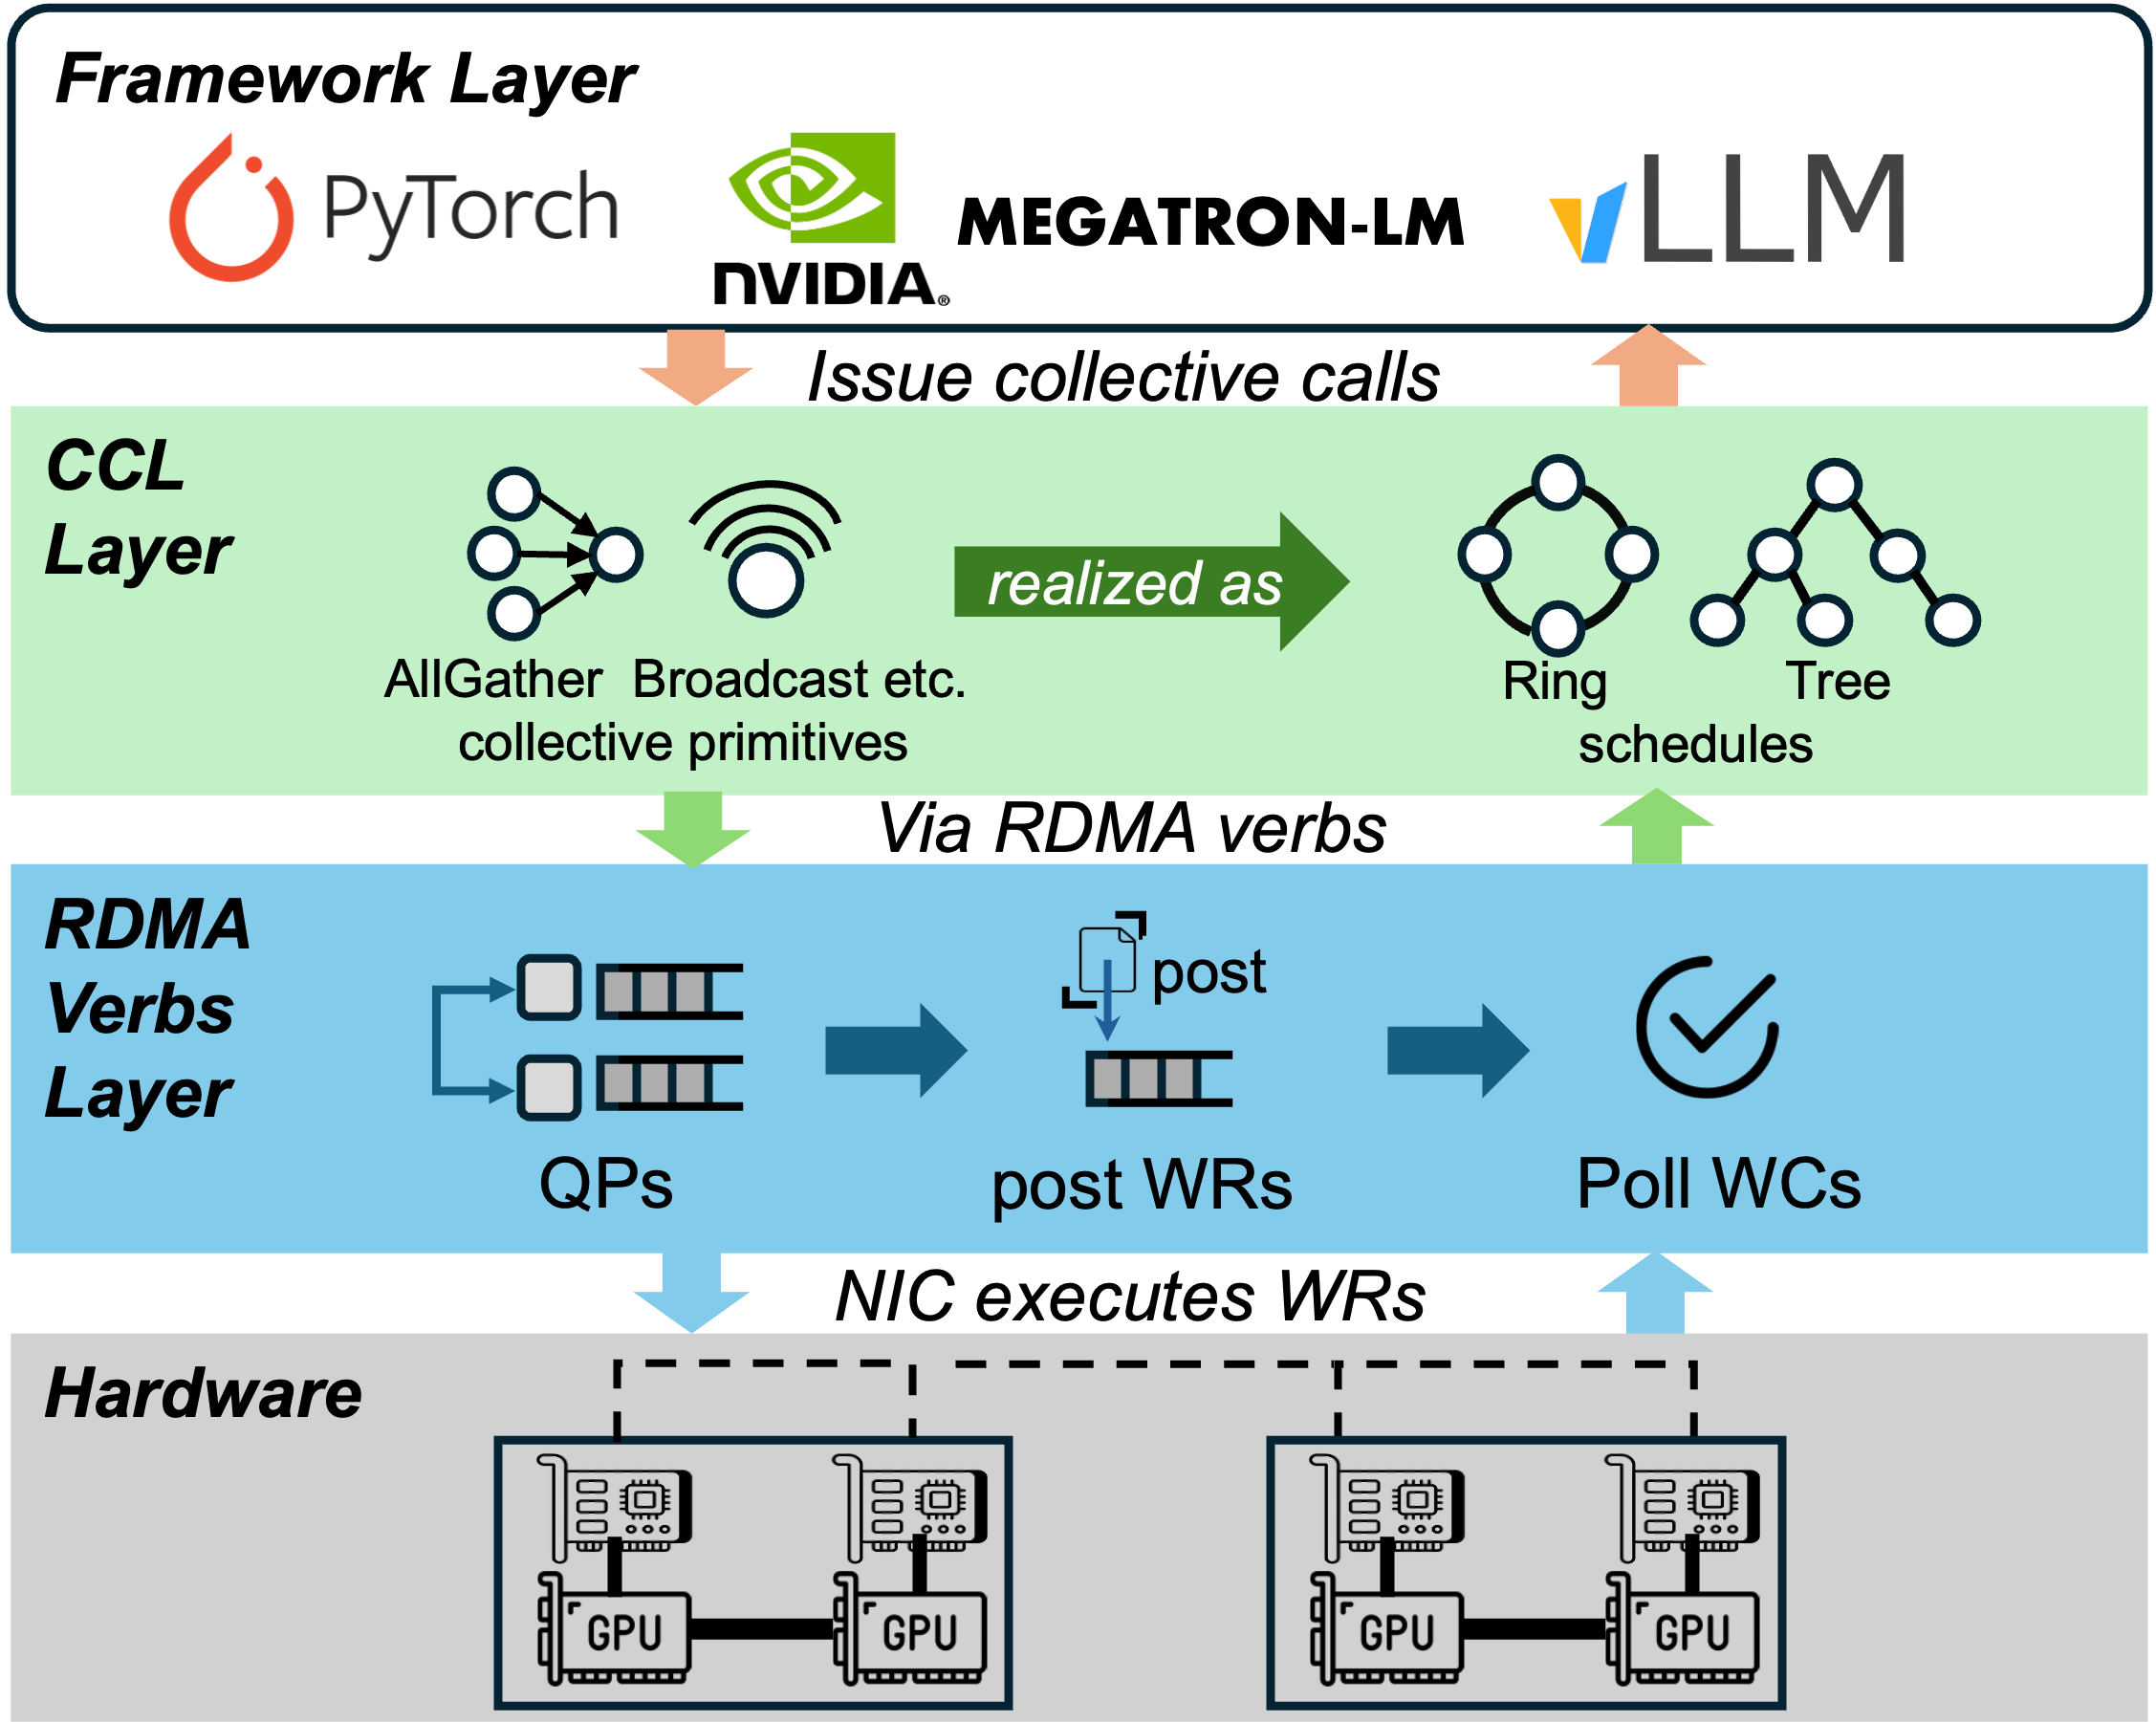
\includegraphics[width=0.97\columnwidth]{figs/new-layer.png}
    \tightcaption{\textbf{Software layering of collective communication.}
    }
    \label{fig:layer}
    \vspace{-3mm}
\end{figure}

\subsection{Current Failure Handling and Limitations}
\label{sec:related}
\noindent\textbf{Framework-level failure handling.} The framework layer handles hardware failures at the granularity of GPU ranks or entire server nodes. Checkpoint-based approaches, such as Gemini~\cite{wang2023gemini} and ByteCheckpoint~\cite{bytecheckpoint}, provide fast in-memory restore, efficient save/load, and resharding across training configurations. Other systems, such as TrainMover~\cite{lao2024trainmover}, use standby machines and live migration to replace failed workers while preserving the training configuration. Oobleck~\cite{oobleck} and ReCycle~\cite{gandhi2024recycle} adapt training execution after worker changes through pipeline templates, replica recovery, or pipeline-schedule adaptation. On the model serving side, D\'{e}j\`{a}Vu~\cite{ICML2024} streams and replicates KV-cache state so that requests can resume on a healthy replica. All of these approaches implicitly assume that the compute endpoint itself is lost or must be removed. As a result, they recover by replacing or excluding entire workers. They are therefore ill-suited for failures where both GPU endpoints remain operational and only a subset of the inter-node network paths is affected.

\smallskip\noindent\textbf{RDMA transport-level failure handling.}
At the RDMA transport layer, failures manifest as queue pair (QP) errors or retry-exhausted operations. For instance, SHIFT~\cite{shift} and LubeRDMA~\cite{luberdma} attempt to mask these failures by transparently reissuing outstanding work requests over alternative paths, allowing transfers to complete without exposing errors to higher layers. However, these mechanisms operate at the level of work requests and completions, without visibility into collective schedules. Under modern low-latency CCL protocols (e.g., LL/LL128 in NCCL~\cite{NCCL}), GPUs may consume data before the corresponding completion is observed by the CPU, which is outside the transport layer's control. As a result, systems like SHIFT~\cite{shift} need to disable low-latency protocols to maintain data correctness at the cost of performance.

\smallskip\noindent\textbf{CCL-layer responses.} At the collective communication layer, mainstream libraries such as NCCL and RCCL have long adopted fail-stop semantics: any transport error aborts the collective, terminates the process, and forces job-level recovery. Although the latest NCCL versions (v2.29.7 and later) support active-active failover across multiple ports or NICs assigned to a GPU, this approach reduces bandwidth as it fails to rebalance collective workloads and schedules. 
Other recent efforts attempt to improve resilience within the CCL layer. For example, AdapCC~\cite{zhao2024adapcc} detects non-responsive workers via timeouts and coordinates with an elastic training controller to continue with a reduced worker set, but it still fails once a fatal error occurs during an ongoing collective. ICCL~\cite{chen2025efficient} pre-establishes primary and backup connections between GPU pairs and migrates traffic upon failure; however, it routes all traffic through a single backup path without adjusting the collective schedule, creating a bottleneck on the affected node.

We observe that \textbf{the key missing piece in today's software stack is a resilient CCL layer.}
Inter-node network failures should be handled within the CCL layer rather than escalating to process or job-level failures. Ideally, the CCL should continue ongoing collectives transparently and correctly, so that collective operations remain indistinguishable from failure-free execution. Beyond merely preserving correctness, it should also adapt communication schedules to the degraded topology and mitigate performance bottlenecks caused by reduced bandwidth. Finally, it should expose degradation signals to upper layers, enabling frameworks to make informed decisions about continuation or recovery, rather than reacting only after a crash occurs.
